
\subsection{Preliminaries}

In this section, we first describe a general probabilistic robot sensing model 
used in this section and introduce the notion of a \emph{continuous monotone 
sweep schedule}, along which robots must be deployed to carry out the 
search task. 
%
Then, the problem of finding the minimum number of robots for a certain 
sweep schedule is formally defined.

\subsubsection{Robot Sensing Model}
\label{sec:sc-sensing}

In this work, a robot is assumed to be a \emph{line guard} capable of sensing 
relevant events happening on a continuous line segment passing through the
robot. 
%
On the line segment guarded by a robot, for a (point) target at a distance 
of $r$ to the robot, the robot has probability $\rho(r)$ of 
detecting or capturing the target, where $\rho: \mathbb{R}^+\rightarrow[0,1]$ 
is a decreasing sensing probability function. 
%define the probability of the robot with line coverage capability
%capturing/detecting a point with distance $r$ to it as $\rho(r)$, where
%$\rho: {R}^+\rightarrow[0,1]$ is a decreasing function. 
%

Individual robots' 1D sensing range aligns to form a \emph{sweep line} or \emph{sweep frontier}.
%
It is assumed that robots carry out their sensing functions independently 
without interfering with each other.
%
For a point $p$ in the sweep line, if it falls between two robots $r_1, r_2$, 
the coverage of that point is provided by $r_1$ and $r_2$, and the 
probability of target detection at that point is computed as $1-(1-\rho(\ell_1))\cdot(1-\rho(\ell_2))=\rho(\ell_1) + \rho(\ell_2) - \rho(\ell_1) \cdot \rho(\ell_2)$, 
where $\ell_1$ (resp., $\ell_2$) is the distance between $p$ and $r_1$ (resp., $r_2$).
%
If it lies at the ends of the segment, the coverage of that point is only provided by the closest robot, 
and the coverage probability is simply $\rho(\ell)$, where $\ell$ is the distance between $p$ and the robot. 
These are illustrated in ~\ref{fig:sc-sensing}.
%
We note that \emph{sweep lines} are not necessarily straight. 
For example, a sweep line could be part of a circle in the case of circular sweeps (~\ref{fig:sc-sweep}(c)).

\begin{figure}[ht]
    \centering
    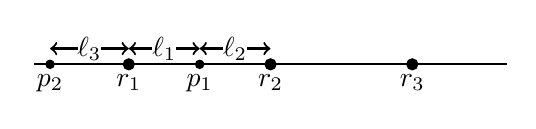
\begin{tikzpicture}
    
        
        \draw[black,thick] (0, 0) -- (6, 0);
        
        \filldraw[black] (0.2, 0) circle (1.5pt)
        node[anchor=north]{$p_2$};
        
        \draw[thick, <-] (0.2, 0.2) -- (0.55, 0.2); 
        \node[] at (0.7,0.2) {$\ell_3$};
        \draw[thick, ->] (0.85, 0.2) -- (1.2, 0.2);
        
        \filldraw[black] (1.2, 0) circle (2pt) node[anchor=north]{$r_1$};
        
        \draw[thick, <-] (1.2, 0.2) -- (1.5, 0.2);
        \node[] at (1.65,0.2) {$\ell_1$};
        \draw[thick, ->] (1.8, 0.2) -- (2.1, 0.2);
        
        \filldraw[black] (2.1, 0) circle (1.5pt)
        node[anchor=north]{$p_1$};
        
        \draw[thick, <-] (2.1, 0.2) -- (2.4, 0.2);
        \node[] at (2.55,0.2) {$\ell_2$};
        \draw[thick, ->] (2.7, 0.2) -- (3, 0.2);
        
        \filldraw[black] (3, 0) circle (2pt) node[anchor=north]{$r_2$};
        
        \filldraw[black] (4.8, 0) circle (2pt) node[anchor=north]{$r_3$};
        
        
    \end{tikzpicture}
    \caption[Illustration of the robot sensing model]
    {Illustration of the robot sensing model. The segment is being covered by three robot guards $r_1 \sim r_3$. The coverage probability of $p_1$, falling between robots $r_1$ and $r_2$, is given as $\rho(\ell_1)+\rho(\ell_2)-\rho(\ell_1)\cdot\rho(\ell_2)$, and the coverage probability of $p_2$, covered only by $r_1$ is given as $\rho(\ell_3)$.}
    \label{fig:sc-sensing}
\end{figure}


For covering a line segment with a length of $\ell$ and sensing function of $\rho$, 
we denote as $\zeta: \mathbb{R}^+ \rightarrow \mathbb{N}^+$ a primitive for computing 
the minimum number of robots needed to achieve the required minimum covering 
probability of $\rho_0$. 
%Denote the primitive as $\zeta: \mathbb{R}^+ \rightarrow \mathbb{N}^+$.

Take the exponential decaying sensing probability function as an example, 
where $\rho(r) = e^{-c\cdot r}$, $c>0$ is some constant.
In this case, the maximum distance at the two ends to guarantee the sensing probability of $\rho_0$ is $d_1=-\ln (\rho_0)/c$. 
If a point is between two robots with distance $\ell_1$ and $\ell_2$ to the two robots, its sensing probability is bounded by

\begin{align*}
\rho(\ell_1) + \rho(\ell_2) - \rho(\ell_1)\cdot \rho(\ell_2)\geq 2e^{-\frac{c\cdot d}{2}} - e^{-c\cdot d}    \\
where\ d = \ell_1+\ell_2
\end{align*}

So, the required maximum distance between two neighboring robots is $d_2=-2\ln(1-\sqrt{1-\rho_0})/c$.
Therefore, the minimum number of robots required to cover a line segment with length $\ell$ is 
$\zeta(\ell) = \max(1, 1 + \lceil(\ell-2\cdot d_1)/d_2 \rceil )$.


\subsection{Problem Formulation}
In this chapter, we work with a 2D compact (i.e., closed and bounded) workspace 
${\mathcal W} \subset \mathbb{R}^2$, which can contain a set of obstacles. 
An existing \emph{sweep schedule} is an input to the problem, which we
define the \emph{continuous monotone sweep schedule} for $\mathcal W$ as 
\begin{definition}[Continuous Monotone Sweep Schedule]
A function $P(t)$ that maps a positive timestamp $t$ to a continuous curve is a continuous monotone sweep schedule for $\mathcal W$ if $P(t)$ changes continuously, 
and for each point $p\in \mathcal W$, there exists a single $t'$ such that $p\in P(t')$.
\end{definition}

Intuitively, a continuous monotone sweep schedule defines a function 
that maps the time step to a 1-D curve in the workspace that sweeps 
through each point in $\mathcal W$ only once. 
%
Depending on the continuous curve, $P(t)$ could take various forms. For example, the sweep line may be straight in a search-and-rescue scenario. Or the sweep line may be circular in a search-and-capture scenario. 
%e a  
%vertical sweeping, circular shrinking, and so on. 
In the rest of this chapter, we simply refer to a continuous monotone sweep schedule as a \emph{sweep schedule}. Next, we introduce the notions of \emph{arrival time} and \emph{monotone chain}.
%
\begin{definition}[Arrival Time]
For a search schedule $P(t)$, and a point in the workspace $o\in\mathcal W$,
the arrival time at $o$, $arrival(o)$, is defined as the time step $t$ when $o\in P(t)$.
\end{definition}

\begin{definition}[Monotone Chain]
For a bounded 2D chain: $\tau(s): [0,1]\rightarrow\mathcal{W}$, where $\tau$ is a continuous function, it is considered as a monotone chain to the search schedule $P(t)$ if and only if
\[s_1 < s_2 \Leftrightarrow arrival(\tau(s_1)) < arrival(\tau(s_2)).\]
\end{definition}
In a search schedule or plan, $P(t)$ may be intersected by obstacles. In this case, $P(t)$ is separated into multiple continuous segments; each of these segments requires a dedicated group of robots. That is, robots on one continuous segment cannot provide coverage of other segments. 

%\r{We may want to define the classes of $\mathcal W$ that we work with. We want to work on a class of environment than can be swept with scan lines. This means that the non-convex obstacles must be able to ``see'' the outside in a some sense.}

With the probabilistic robot sensing model, we formulate the robot team scheduling problem for a given sweep schedule as the following,
\begin{problem}
Given a sweep schedule $P(t)$ for a 2D region $\mathcal W$, and a group of robots with coverage capability function $\rho$, what is the minimum number of robots required to execute the sweep schedule on the sweep line, such that 
for every point $o$ in $\mathcal W$, the probability that $o$ is covered is at 
least some fixed $0 < \rho_0 \le 1$?
\end{problem}

